\documentclass[12pt,a4paper]{article}
\usepackage{amsmath}
\usepackage{graphicx}

\begin{document}
	
% Folha de rosto
\begin{titlepage}
	\centering
	\vspace{2cm}
	
	{UNIVERSIDADE FEDERAL FLUMINENSE} \\ [0.1cm]
	{BACHARELADO EM CIÊNCIA DA COMPUTAÇÃO} \\ [0.1cm]
	{TCC00288 - BANCO DE DADOS II}
	
	\vfill
	
	{\Large \bfseries Avaliação Continuada 2: Particionamento de Tabelas}
	
	\vfill
	
	{BEATRIZ DE OLIVEIRA PIEDADE}
	
	\vfill
	{NITERÓI} \\
	{2024}
\end{titlepage}

\tableofcontents

% Conteúdo
\newpage
\section{Esquema}

\begin{flushleft}
	Pessoa (\underline{CodPessoa}, Nome, Idade, UF) \\[0.2cm]
	Receita (\underline{CodReceita}, DataPostagem, Título, ModoPreparo, CodPessoa) \\
	\quad \quad \quad \quad CodPessoa REFERENCIA Pessoa(CodPessoa) \\[0.2cm]
	
	Ingrediente (\underline{CodIngrediente}, Descrição, Unidade) \\[0.2cm]
	IngredienteReceita (\underline{CodReceita, CodIngrediente}, Quantidade) \\
	\quad \quad \quad \quad CodReceita REFERENCIA Receita (CodReceita) \\
	\quad \quad \quad \quad CodIngrediente REFERENCIA Ingrediente (CodIngrediente) \\[0.2cm]
\end{flushleft}

\newpage
\section{Predicados Simples}

Considerando as seguintes consultas frequentes a esse banco de dados:

\begin{description}
	\item - Códigos das receitas postadas por pessoas com menos de 14 anos
	\begin{verbatim}
		SELECT Receita.CodReceita
		FROM Receita
		JOIN Pessoa
		ON Receita.CodPessoa = Pessoa.CodPessoa
		WHERE Pessoa.Idade < 14
	\end{verbatim}
	
	\item - Códigos das receitas que foram postadas por pessoas com mais de 18 anos
	\begin{verbatim}
		SELECT Receita.CodReceita
		FROM Receita
		JOIN Pessoa
		ON Receita.CodPessoa = Pessoa.CodPessoa
		WHERE Pessoa.Idade > 18
	\end{verbatim}
	
	\item - Nomes das pessoas que residem no Rio de Janeiro (UF = "RJ")
	\begin{verbatim}
		SELECT Pessoa.Nome
		FROM Pessoa
		WHERE Pessoa.UF = 'RJ'
	\end{verbatim}
	
	\item - Nomes das pessoas que residem em São Paulo (UF = "SP")
	\begin{verbatim}
		SELECT Pessoa.Nome
		FROM Pessoa
		WHERE Pessoa.UF = 'SP'
	\end{verbatim}
\end{description}

\noindent
Os predicados simples são:
\begin{description}
	\item[P1.] Idade $<$ 14
	\item[P2.] Idade $>$ 18
	\item[P3.] UF = $'RJ'$
	\item[P4.] UF = $'SP'$
\end{description}
	
\newpage
\section{Representação Dono x Membro}

Observando a representação Dono x Membro das tabelas da aplicação:

\begin{center}
	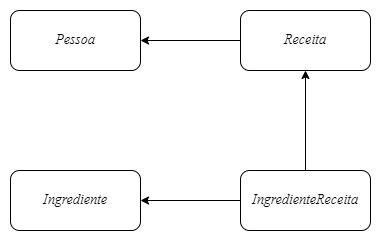
\includegraphics[width=180px]{diagrama.jpg}
\end{center}

As tabelas \textit{Pessoa} e \textit{Ingrediente} adotarão a Fragmentação Horizontal Primária (FHP) e as tabelas \textit{Receita} e \textit{IngredienteReceita} adotarão a Fragmentação Horizontal Derivada (FHD)

\newpage
\section{Fragmentação Horizontal}

\subsection{FHP de Pessoa}

\begin{flushleft}
Os predicados simples associados a tabela Pessoa são:
\begin{description}
	\item[P1.] Idade $<$ 14
	\item[P2.] Idade $>$ 18
	\item[P3.] UF = $'RJ'$
	\item[P4.] UF = $'SP'$ 
\end{description}
\end{flushleft}

\noindent
\begin{flushleft}
Logo, os mintermos são:
\begin{description}
	\item[M1.] P1 $\wedge$ P2 $\wedge$ P3 $\wedge$ P4
	\item[M2.] P1 $\wedge$ P2 $\wedge$ P3 $\wedge$ \textlnot P4
	\item[M3.] P1 $\wedge$ P2 $\wedge$ \textlnot P3 $\wedge$ P4
	\item[M4.] P1 $\wedge$ \textlnot P2 $\wedge$ P3 $\wedge$ P4
	\item[M5.] \textlnot P1 $\wedge$ P2 $\wedge$ P3 $\wedge$ P4
	\item[M6.] P1 $\wedge$ P2 $\wedge$ \textlnot P3 $\wedge$ \textlnot P4
	\item[M7.] P1 $\wedge$ \textlnot P2 $\wedge$ P3 $\wedge$ \textlnot P4
	\item[M8.] \textlnot P1 $\wedge$ P2 $\wedge$ P3 $\wedge$ \textlnot P4
	\item[M9.] P1 $\wedge$ \textlnot P2 $\wedge$ \textlnot P3 $\wedge$ P4
	\item[M10.] \textlnot P1 $\wedge$ P2 $\wedge$ \textlnot P3 $\wedge$ P4
	\item[M11.] \textlnot P1 $\wedge$ \textlnot P2 $\wedge$ P3 $\wedge$ P4
	\item[M12.] P1 $\wedge$ \textlnot P2 $\wedge$ \textlnot P3 $\wedge$ \textlnot P4
	\item[M13.] \textlnot P1 $\wedge$ P2 $\wedge$ \textlnot P3 $\wedge$ \textlnot P4
	\item[M14.] \textlnot P1 $\wedge$ \textlnot P2 $\wedge$ P3 $\wedge$ \textlnot P4
	\item[M15.] \textlnot P1 $\wedge$ \textlnot P2 $\wedge$ \textlnot P3 $\wedge$ P4
	\item[M16.] \textlnot P1 $\wedge$ \textlnot P2 $\wedge$ \textlnot P3 $\wedge$ \textlnot P4
\end{description}
\end{flushleft}

\noindent
\begin{flushleft}
Observando as implicações geradas pelos predicados simples:
\begin{description}
	\item (P1: Idade $<$ 14) $\longrightarrow$ \textlnot (P2: Idade $>$ 18)
	\item (P2: Idade $>$ 18) $\longrightarrow$ \textlnot (P1: Idade $<$ 14) 
	\item (P3: UF = $'RJ'$) $\longrightarrow$ \textlnot (P4: UF = $'SP'$)
	\item (P4: UF = $'SP'$) $\longrightarrow$ \textlnot (P3: UF = $'RJ'$)
\end{description}
\end{flushleft}

\noindent
\begin{flushleft}
	Logo, os mintermos válidos são:
	\begin{description}
		\item[M7.] (Idade $<$ 14) $\wedge$ \textlnot (Idade $>$ 18) $\wedge$ (UF = $'RJ'$) $\wedge$ \textlnot (UF = $'SP'$)
		\item[M8.] \textlnot (Idade $<$ 14) $\wedge$ (Idade $>$ 18) $\wedge$ (UF = $'RJ'$) $\wedge$ \textlnot (UF = $'SP'$)
		\item[M9.] (Idade $<$ 14) $\wedge$ \textlnot (Idade $>$ 18) $\wedge$ \textlnot (UF = $'RJ'$) $\wedge$ (UF = $'SP'$)
		\item[M10.] \textlnot (Idade $<$ 14) $\wedge$ (Idade $>$ 18) $\wedge$ \textlnot (UF = $'RJ'$) $\wedge$ (UF = $'SP'$)
		\item[M12.] (Idade $<$ 14) $\wedge$ \textlnot (Idade $>$ 18) $\wedge$ \textlnot (UF = $'RJ'$) $\wedge$ \textlnot (UF = $'SP'$)
		\item[M13.] \textlnot (Idade $<$ 14) $\wedge$ (Idade $>$ 18) $\wedge$ \textlnot (UF = $'RJ'$) $\wedge$ \textlnot (UF = $'SP'$)
		\item[M14.] \textlnot (Idade $<$ 14) $\wedge$ \textlnot (Idade $>$ 18) $\wedge$ (UF = $'RJ'$) $\wedge$ \textlnot (UF = $'SP'$)
		\item[M15.] \textlnot (Idade $<$ 14) $\wedge$ \textlnot (Idade $>$ 18) $\wedge$ \textlnot (UF = $'RJ'$) $\wedge$ (UF = $'SP'$)
		\item[M16.] \textlnot (Idade $<$ 14) $\wedge$ \textlnot (Idade $>$ 18) $\wedge$ \textlnot (UF = $'RJ'$) $\wedge$ \textlnot (UF = $'SP'$)
	\end{description}
\end{flushleft}

\noindent
\begin{flushleft}
	Os fragmentos resultantes são:
	\begin{description}
		\item[Pessoa1 =] $\sigma$ (Idade $<$ 14 $\wedge$ UF = $'RJ'$) Pessoa
		\item[Pessoa2 =] $\sigma$ (Idade $>$ 18 $\wedge$ UF = $'RJ'$) Pessoa
		\item[Pessoa3 =] $\sigma$ (Idade $<$ 14 $\wedge$ UF = $'SP'$) Pessoa
		\item[Pessoa4 =] $\sigma$ (Idade $>$ 18 $\wedge$ UF = $'SP'$) Pessoa
		\item[Pessoa5 =] $\sigma$ (Idade $<$ 14 $\wedge$ UF != $'RJ'$ $\wedge$ UF != $'SP'$) Pessoa
		\item[Pessoa6 =] $\sigma$ (Idade $>$ 18 $\wedge$ UF != $'RJ'$ $\wedge$ UF != $'SP'$) Pessoa
		\item[Pessoa7 =] $\sigma$ (Idade $>=$ 14 $\wedge$ Idade $<=$ 18 $\wedge$ UF = $'RJ'$) Pessoa
		\item[Pessoa8 =] $\sigma$ (Idade $>=$ 14 $\wedge$ Idade $<=$ 18 $\wedge$ UF = $'SP'$) Pessoa
		\item[Pessoa9 =] $\sigma$ (Idade $>=$ 14 $\wedge$ Idade $<=$ 18 $\wedge$ UF != $'RJ'$ $\wedge$ UF != $'SP'$) Pessoa
	\end{description}
\end{flushleft}

\subsection{FHP de Ingrediente}

Tendo em vista que nenhuma das consultas frequentes envolve um predicado relacionado à tabela Ingrediente, não é necessário fragmentá-la.

\subsection{FHD de Receita}

Como a tabela Receita está relacionada à tabela Pessoa, que já foi fragmentada horizontalmente, sua fragmentação será derivada dela.

\begin{flushleft}
	\begin{description}
		\item[Receita1 =] Receita $\bowtie$ Pessoa1
		\item[Receita2 =] Receita $\bowtie$ Pessoa2
		\item[Receita3 =] Receita $\bowtie$ Pessoa3
		\item[Receita4 =] Receita $\bowtie$ Pessoa4
		\item[Receita5 =] Receita $\bowtie$ Pessoa5
		\item[Receita6 =] Receita $\bowtie$ Pessoa6
		\item[Receita7 =] Receita $\bowtie$ Pessoa7
		\item[Receita8 =] Receita $\bowtie$ Pessoa8
		\item[Receita9 =] Receita $\bowtie$ Pessoa9
	\end{description}
\end{flushleft}

\subsection{FHD de IngredienteReceita}

Tendo em vista que nenhuma das consultas frequentes envolve um predicado relacionado à tabela IngredienteReceita, não é necessário fragmentá-la.
\end{document}
